\chapter[Hybrid Quantum-Classical Algorithms]{Hybrid Quantum-Classical\\Algorithms} \label{chap:hybrid-quantum-classical-algorithms}
At the end of the previous chapter, two important quantum algorithms were reviewed: the \gls{qft} and Grover's algorithm.
These quantum algorithms and the family of algorithms built on them require large-scale quantum computers with low error rates and high coherence.
The \gls{nisq} devices that are being built now and in the near future will not be able to run these algorithms due to their limited qubit count, limited coherence times, and high error rates.
To this end, \acrfullpl{hqca} that utilize both classical and quantum resources are being researched and developed.
This chapter will first introduce the basic concepts of an important family of \glspl{hqca} followed by a review of well-known and promising \glspl{hqca}.

\section{Variational Hybrid Quantum-Classical Algorithms}
\Acrlongpl{hqca} take into account the limited number of qubits, limited connectivity of qubits, high error rates, and limited coherence times of \gls{nisq} devices.
These algorithms often make use of the variational method which consists of preparing an initial trial state $\ket{\psi(\vec{\theta})}$ parameterized by real-valued parameters $\vec{\theta}$, and finding the parameters for which the expectation value of some observable is the lowest.
This family of \glspl{hqca} is sometimes also referred to as variational quantum algorithm, as it uses the variational method of quantum mechanics.
The rest of this chapter will be focused on variational \glspl{hqca}, as this is the main focus of research regarding \glspl{hqca}.

The general structure of a variational \gls{hqca} is shown in \Cref{fig:vqa-general-structure}.
While the specific implementation differs between algorithms, they all share some basic elements.
First, a cost function $C$ which encodes the solution to the problem needs to be defined.
Second, an ansatz needs to be chosen.
The ansatz defines the operations of the quantum circuit which are parameterized by the trainable parameters $\vec{\theta}$.
\begin{figure}[ht]
    \centering
    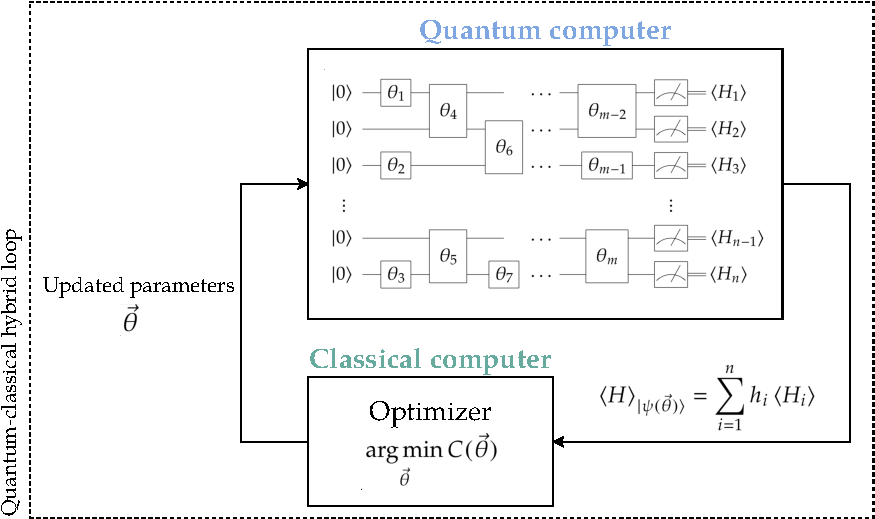
\includegraphics[width=1\linewidth]{figures/vqa-general-structure.pdf}
    \caption[The general structure of a variational \acrshort{hqca}.]{The general structure of a variational \gls{hqca}. A parameterized quantum state $\ket{\psi(\vec{\theta})}$ is prepared through a set of parameterized quantum gates $U_L(\vec{\theta}_L) \ldots U_2(\vec{\theta}_2)U_1(\vec{\theta}_1)$. These parameters are classically optimized according to a cost function $C(\vec{\theta})$. This quantum-classical loop is repeated until convergence.}
    \label{fig:vqa-general-structure}
\end{figure}
The parameters $\vec{\theta}$ are then trained in a quantum-classical loop to solve the optimization problem
\begin{equation} \label{eqn:optimization-problem}
\argmin_{\vec{\theta}} C(\vec{\theta}).
\end{equation}

\subsection{Cost Function}
In general, the cost function has the form
\begin{equation} \label{eqn:general-cost-function}
C(\vec{\theta}) = \sum_k f_k\left(\bra{0^n}U(\vec{\theta})^\dagger H_k U(\vec{\theta})\ket{0^n}\right),
\end{equation}
where $f_k$ is a function encoding the problem at hand, $U(\vec{\theta})$ is the quantum circuit parameterized by real values $\vec{\theta}$, $H_k$ is an observable, and $n$ is the number of qubits.
A key point of variational \glspl{hqca} is that a quantum computer is used to estimate $C(\vec{\theta})$ while using a classical computer to optimize the parameters $\vec{\theta}$.
Furthermore, the cost function $C(\vec{\theta})$ should be efficient to estimate by performing measurements on a quantum computer.
For the variational \gls{hqca} to have a quantum advantage, the cost should also not be efficiently computable with a classical computer.

\subsection{Ans{\"a}tze}
The ansatz defines the quantum circuit $U(\vec{\theta})$ that is used to prepare the quantum state $\ket{\psi(\vec{\theta})}$ parameterized by real-valued parameters $\vec{\theta}$.
To keep the algorithm realizable on \gls{nisq} devices, it is important to keep the parameterized quantum circuit (the ansatz) relatively shallow in depth.
The challenge then is to choose an ansatz that is shallow in depth but has high expressibility.
\textcite{sim2019expressibility} define the expressibility of a quantum circuit as its ability to generate states that are well representative of the Hilbert space.
The general form of an ansatz can be described as the product of sequentially applied unitaries:
\begin{equation}
U(\vec{\theta}) = U_L(\vec{\theta}_L) \ldots U_2(\vec{\theta}_2)U_1(\vec{\theta}_1),
\end{equation}
where
\begin{equation} \label{eqn:ansatz-unitary}
U_l(\vec{\theta}_l) = \prod_{m} e^{-i \tfrac{\theta_m}{2} H_m}W_m.
\end{equation}
Here $H_m$ is a Hermitian operator and $W_m$ is a non-parameterized unitary.
\Cref{eqn:ansatz-unitary} can simply be thought of as alternating between parameterized and non-parameterized unitaries.

The specific structure of the ansatz usually depends on the problem, as one can sometimes employ information about the problem to tailor an ansatz~\cite{cerezo2020variational}.
Such ans{\"a}tze are referred to as problem-inspired ans{\"a}tze.
On the other hand, there are problem-agnostic ans{\"a}tze that are used when no information is available for tailoring a specific ansatz.

\subsection{Optimization}
With the cost function and ansatz defined, the next step in a variational \gls{hqca} is to train the parameters $\vec{\theta}$ using a classical optimization algorithm to solve the optimization problem from \Cref{eqn:optimization-problem}.
The two main types of optimization methods to consider are gradient-based methods and gradient-free methods.
The former methods involve calculating first- or higher-order derivatives of the cost function, while the latter methods use only function evaluations.
In general, the computational cost of gradient-based methods is larger, but the rate of convergence is significantly improved.

While gradient-free methods are straightforward to use for optimizing the quantum circuit parameters, gradient-based methods are more involved.
Consider a parameterized gate $G(\theta) = e^{-i\theta/2 H}$ from the general ansatz description in \Cref{eqn:ansatz-unitary}.
Using the parameter-shift rule as described by \textcite{schuld2019evaluating}, the derivative of the gate $G$ with respect to a parameter $\theta$ can be described as follows:
\begin{equation}
\dfrac{\partial G}{\partial \theta} = \dfrac{1}{2}\left[G\left(\theta + \dfrac{\pi}{2}\right) - G\left(\theta - \dfrac{\pi}{2}\right)\right].
\end{equation}
That is, the derivative of $G$ with respect to a parameter $\theta$ can be computed analytically by evaluating the quantum circuit twice with shifted parameters $\theta \pm \pi/2$.
In term, the derivative of a cost function $C(\vec{\theta}) = \sum_k \bra{0^n}U(\vec{\theta})^\dagger H_k U(\vec{\theta})\ket{0^n}$ with respect to a parameter $\theta_l$ can be estimated as follows:
\begin{equation}
\begin{aligned}
\dfrac{\partial C}{\partial \theta_l} = \sum_k \dfrac{1}{2} \bigg[&\bra{0^n}U\left(\vec{\theta} + \dfrac{\pi}{2}\vec{e}_l\right)^\dagger H_k U\left(\vec{\theta} + \dfrac{\pi}{2}\vec{e}_l\right)\ket{0^n} \\
- \; &\bra{0^n}U\left(\vec{\theta} - \dfrac{\pi}{2}\vec{e}_l\right)^\dagger H_k U\left(\vec{\theta} - \dfrac{\pi}{2}\vec{e}_l\right)\ket{0^n}\bigg],
\end{aligned}
\end{equation}
where $\vec{e}_l$ is a vector with $1$ as its $l$-th element and $0$ for all other elements.
The parameter-shift rule can be further generalized to calculate higher-order derivatives of quantum gates~\cite{mari2021estimating}, allowing the use of optimization methods that use higher-order derivates such as Newton's method.

A common way to perform optimization is through gradient descent based algorithms.
Gradient descent uses first-order derivatives for finding a local minimum of a differentiable function.
Intuitively, it takes repeated steps in the opposite direction of the gradient of the function until the gradient is zero~(\Cref{fig:gradient_descent}).
Formally, for a set of parameters $\vec{\theta}_t$ and a cost function $C(\vec{\theta})$, the updated parameters $\vec{\theta}_{t+1}$ after one iteration of gradient descent is as follows:
\begin{equation}
\vec{\theta}_{t+1} = \vec{\theta}_t - \eta\nabla C(\vec{\theta}_t),
\end{equation}
where $\eta$ is the step size which determines how big of a step the algorithm makes each iteration.
The step size impacts the performance of the algorithm: if it is too large the optimization algorithm will diverge, and if it is too small it will take a long time to converge.
The gradient descent based optimization algorithm Adam adapts the step size during optimization to increase the efficiency and accuracy of solutions~\cite{kingma2014adam}.

\begin{figure}[ht]
    \centering
    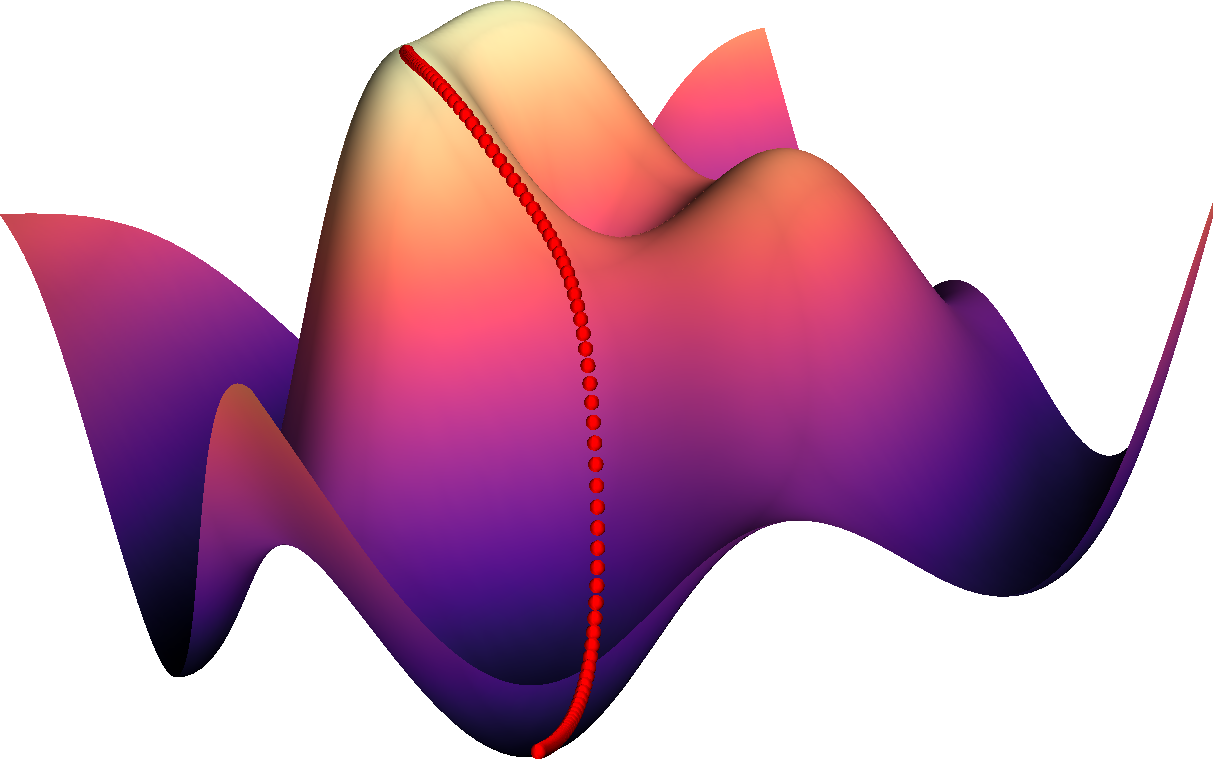
\includegraphics[width=0.6\linewidth]{figures/gradient_descent.png}
    \caption[Visualization of gradient descent finding a local minimum of a function.]{Visualization of gradient descent finding a local minimum of a two-dimensional function. The two parameters start at the top of the function landscape and gradually find a local minimum by moving in the opposite direction of the gradient.}
    \label{fig:gradient_descent}
\end{figure}

\section{Variational Quantum Eigensolver}
The \gls{vqe} was the first proposed variational \gls{hqca}.
It aims to solve the problem of finding eigenvalues of a Hamiltonian $H$.
The problem of finding eigenvalues for large matrices has applications in quantum chemistry, but potential applications range from determining the results of search engines~\cite{page1999pagerank} to designing new materials and drugs~\cite{golub2000eigenvalue}.
A previously known quantum algorithm called the \gls{qpea} solves this problem exponentially faster than the best known classical algorithm~\cite{abrams1999quantum}.
However, the quantum resources required to run the \gls{qpea} greatly exceed the resources available in the near term.
\textcite{peruzzo2014variational} proposed the \gls{vqe} as alternative which can run on \gls{nisq} devices.

Formally, the \gls{vqe} estimates the minimum eigenvalue $\lambda_{\textnormal{min}}$ associated with eigenstate $\ket{\lambda_{\textnormal{min}}}$ for a Hermitian operator $H$.
The cost function is defined as the expectation value of $H$ over a trial state $\ket{\psi({\vec{\theta}})} = U(\vec{\theta})\ket{\psi_0}$ where $U(\vec{\theta})$ is the ansatz and $\ket{\psi_0}$ an initial guess state:
\begin{equation}
C(\vec{\theta}) = \bra{\psi(\vec{\theta})}H\ket{\psi(\vec{\theta})}.
\end{equation}
Minimizing this cost function estimates the minimum eigenvalue of $H$, as the Rayleigh-Ritz variational principle provides the following bound~\cite{ritz1909neue}:
\begin{equation}
\lambda_{\textnormal{min}} \leq \bra{\psi(\vec{\theta})}H\ket{\psi(\vec{\theta})}.
\end{equation}
That is, a trial state $\ket{\psi({\vec{\theta}})}$ will always give an expectation value larger than or equal to the minimum eigenvalue.
In the context of quantum chemistry, where $H$ describes the Hamiltonian of a system, finding the lowest eigenvalue of the Hamiltonian translates to finding the ground state energy of that system.
By selecting an initial guess state, calculating the expectation value of $H$, and optimizing the cost function $C(\vec{\theta})$, one can then approximate the ground state energy of a Hamiltonian to arbitrary precision.

% efficient on quantum computer - hard on classical - measuring of <H>

\section{Quantum Approximate Optimization Algorithm}